\documentclass{standalone}
\usepackage{tikz}
\usetikzlibrary{arrows.meta}

% Define arrow colors
\tikzset{
    greenarrow/.style={->, line width=1.5pt, green!70!black},
    bluearrow/.style={->, line width=1.5pt, blue!80!black},
    redarrow/.style={->, line width=1.5pt, red!80!black},
    orangearrow/.style={->, line width=1.5pt, orange!80!black},
    cyanarrow/.style={->, line width=1.5pt, cyan!80!black},
    blackarrow/.style={->, line width=1.5pt, black},
}

\begin{document}
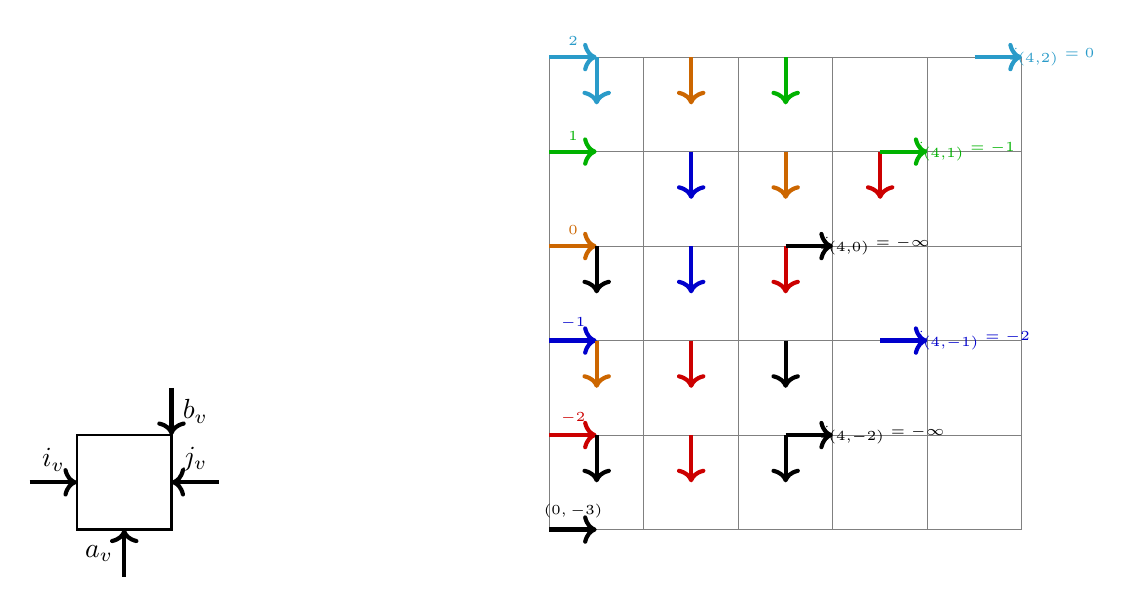
\begin{tikzpicture}[scale=1.2]

% Left part: Vertex labels
\draw[thick] (0,0) -- (1,0) -- (1,1) -- (0,1) -- cycle;
\draw[blackarrow] (-0.5,0.5) -- (0,0.5) node[pos=0.5, above] {$i_v$};
\draw[blackarrow] (1,1.5) -- (1,1) node[pos=0.5, right] {$b_v$};
\draw[blackarrow] (1.5,0.5) -- (1,0.5) node[pos=0.5, above] {$j_v$};
\draw[blackarrow] (0.5,-0.5) -- (0.5,0) node[pos=0.5, left] {$a_v$};

% Right part: Stochastic six-vertex model
\begin{scope}[xshift=5cm]
    % Draw the grid
    \foreach \x in {0,...,5} {
        \draw[gray] (\x,0) -- (\x,5);
    }
    \foreach \y in {0,...,5} {
        \draw[gray] (0,\y) -- (5,\y);
    }

    % Add horizontal arrows
    \draw[cyanarrow] (0,5) -- (0.5,5) node[pos=0.5, above] {\tiny$2$};
    \draw[greenarrow] (0,4) -- (0.5,4) node[pos=0.5, above] {\tiny$1$};
    \draw[orangearrow] (0,3) -- (0.5,3) node[pos=0.5, above] {\tiny$0$};
    \draw[bluearrow] (0,2) -- (0.5,2) node[pos=0.5, above] {\tiny$-1$};
    \draw[redarrow] (0,1) -- (0.5,1) node[pos=0.5, above] {\tiny$-2$};
    \draw[blackarrow] (0,0) -- (0.5,0) node[pos=0.5, above] {\tiny$(0,-3)$};

    % Add vertical arrows
    \draw[cyanarrow] (0.5,5) -- (0.5,4.5);
    \draw[orangearrow] (1.5,5) -- (1.5,4.5);
    \draw[greenarrow] (2.5,5) -- (2.5,4.5);

    \draw[bluearrow] (1.5,4) -- (1.5,3.5);
    \draw[orangearrow] (2.5,4) -- (2.5,3.5);
    \draw[redarrow] (3.5,4) -- (3.5,3.5);

    \draw[blackarrow] (0.5,3) -- (0.5,2.5);
    \draw[bluearrow] (1.5,3) -- (1.5,2.5);
    \draw[redarrow] (2.5,3) -- (2.5,2.5);

    \draw[orangearrow] (0.5,2) -- (0.5,1.5);
    \draw[redarrow] (1.5,2) -- (1.5,1.5);
    \draw[blackarrow] (2.5,2) -- (2.5,1.5);

    \draw[blackarrow] (0.5,1) -- (0.5,0.5);
    \draw[redarrow] (1.5,1) -- (1.5,0.5);
    \draw[blackarrow] (2.5,1) -- (2.5,0.5);

    % Add horizontal arrows (right side)
    \draw[cyanarrow] (4.5,5) -- (5,5) node[pos=0.5, right] {\tiny$j_{(4,2)} = 0$};
    \draw[greenarrow] (3.5,4) -- (4,4) node[pos=0.5, right] {\tiny$j_{(4,1)} = -1$};
    \draw[blackarrow] (2.5,3) -- (3,3) node[pos=0.5, right] {\tiny$j_{(4,0)} = -\infty$};
    \draw[bluearrow] (3.5,2) -- (4,2) node[pos=0.5, right] {\tiny$j_{(4,-1)} = -2$};
    \draw[blackarrow] (2.5,1) -- (3,1) node[pos=0.5, right] {\tiny$j_{(4,-2)} = -\infty$};
\end{scope}
\end{tikzpicture}
\end{document}